\section{Auswertung}
\label{sec:Auswertung}
Für die Untersuchung der verschiedenen aufgenommenen $\gamma$-Spektren werden die Kanäle des ``VKA'' auf die entsprechenden Energien kalibriert. Desweiteren wird die Effizienz des Detektors an dem $^{152}$Eu-Spektrum berechnet und anschließend die Messwerte zur Bestimmung der Aktivität der verwendeten $^{133}$Bariumquelle mit ihr bereinigt. Desweiteren wird das Compton-Kontinum sowie der Photopeak einer $^{137}$Cs-Quelle untersucht, sowie geprüft ob der Photopeak gaußverteilt ist. Zuletzt wird anhand des Spektrums versucht auf die Zerfallsprodukte eines Minerals zu schließen und somit deren Zerfallskette zu bestimmen.


\subsection{Kalibrieren des Detektors anhand $^{152}$Eu Spektrums}
Zum kalibrieren des Detektors werden im Folgenden den Kanalnummern die entsprechenden Energien zugewiesen, sowie die Effizienz des Detektors bestimmt. Dazu wurde bei einer Messzeit von 3172 Sekunden das Spektrum, welches in Abbildung \ref{fig:spekEu} zu sehen ist, aufgenommen.
\begin{figure}[H]
  \centering
  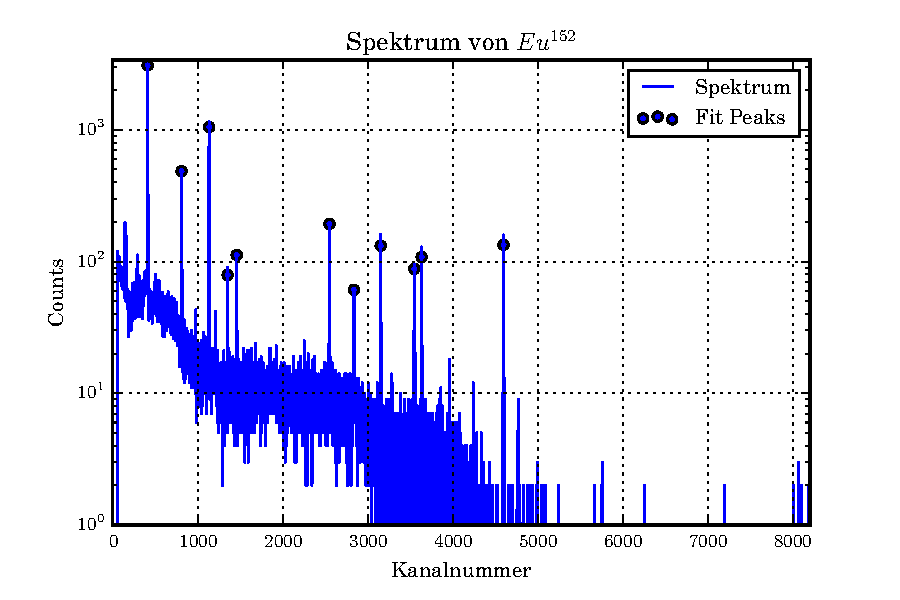
\includegraphics[width=\textwidth]{./Bilder/SpektEu.pdf}
  \caption{Unkalibriertes Spektrum des $^{152}$Eu-Strahlers}
  \label{fig:spekEu}
\end{figure}

\subsubsection{Energiekalibrierung}
\label{sec:Kalb}
Zunächst wird die Kanalnummer auf die Energie, anhand des Spektrums des $^{152}$Eu-Strahlers, kalibriert. Die Energie mit den entsprechenden Kanalnummern sind in Tabelle \ref{tab:CsSpekt} aufgeführt. Die Kanalnummern werden aus den Hochpunkten der durch die Peaks gefitteten Gaußfunktion bestimmt. Als Unsicherheit auf die Kanalnummer, wird die Standardabweichung der Gaußfunktion genommen.

\begin{table}[H]
  \centering
  \caption{Kenngrößen eines $^{152}$Eu-Strahlers, sowie des Detektors}
  \begin{tabular}{c | c c }
    \toprule
    Energie $E_{\gamma}$ / keV \cite{V18}& Kanal & $E_{Exp}$ / keV \\
    \hline
    121,78  & \num{403 +- 1,5}	& \num{121,81 +- 0,07}	\\
    244,70  & \num{803 +- 1,7}  & \num{244,60 +- 0,07}	\\
    344,30  & \num{1128+- 1,7}	& \num{344,37 +- 0,08}	\\
    411,12  & \num{1345+- 2,2}	& \num{410,98 +- 0,08}	\\
    443,96  & \num{1452+- 2,0}	& \num{443,98 +- 0,08}	\\
    778,90  & \num{2544+- 2,4}	& \num{779,04 +- 0,10}	\\
    867,37  & \num{2832+- 2,7}	& \num{867,45 +- 0,10}	\\
    964,08  & \num{3147+- 2,5}	& \num{964,15 +- 0,11}	\\
    1085,90 & \num{3543+- 2,5}	& \num{1085,71 +- 0,12}	\\
    1112,10 & \num{3629+- 2,5}	& \num{1112,11 +- 0,12}	\\
    1408,00 & \num{4593+- 2,5}	& \num{1408,03 +- 0,14}	\\
    \bottomrule
  \end{tabular}
  \label{tab:CsSpekt}
\end{table}

Um die Korrelation zwischen der Energie und der Kanalnummer zu bestimmen wird eine lineare Regression durch elf Tupel aus Energie und Kanalnummer gelegt. Diese werden mit den Fehlern den Standardabweichungen der Kanalnummern gewichtet. Das Ergebnis ist in Abbildung \ref{fig:RegEu} zu sehen.

\begin{figure}[H]
  \centering
  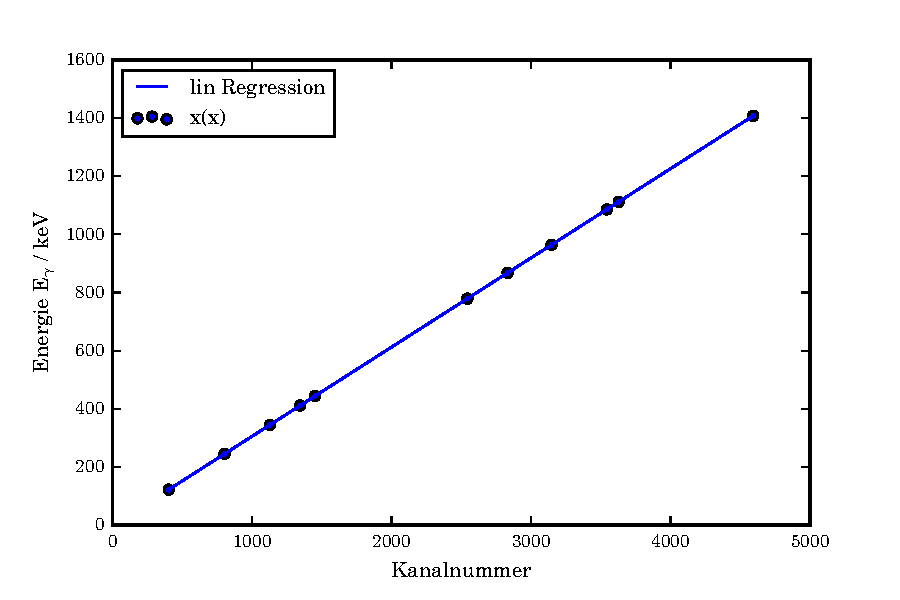
\includegraphics[width=\textwidth]{./build/CsReg.pdf}
  \caption{Lineare Regression zur Bestimmung der Korrelation zwischen Kanalnummer und $\gamma$-Quantenenergie}
  \label{fig:RegEu}
\end{figure}

Aus der linearen Regression ergibt sich eine Steigung von
\begin{equation}
  \Delta E = (\num{306,97 +- 0,03}) \, \text{eV}
  \label{eqn:Reg}
\end{equation}
sowie eine Bios von
\begin{equation}
  E_\text{Bios} = (\num{-1910 +- 60}) \, \text{eV} \ .
  \label{eqn:Bios}
\end{equation}
Anhand der Energieskala werden die gemessenen Counts im weiteren in Abhängikeit der $\gamma$-Quanten Energie $E_{\gamma}$ dargestellt. In Tabelle \ref{tab:CsSpekt} sind die Energien die sich anhand der ermittelten Parametern und der Lage der Peaks ergeben und der Literaturwert aufgeführt.


\subsubsection{Effizienzbestimmung}
\label{sec:Q}
Das für den $^{152}$Eu-Strahler aufgenommene Spektrum ist in Abbildung \ref{fig:SpekCs} zu sehen.
\begin{figure}[h]
  \centering
  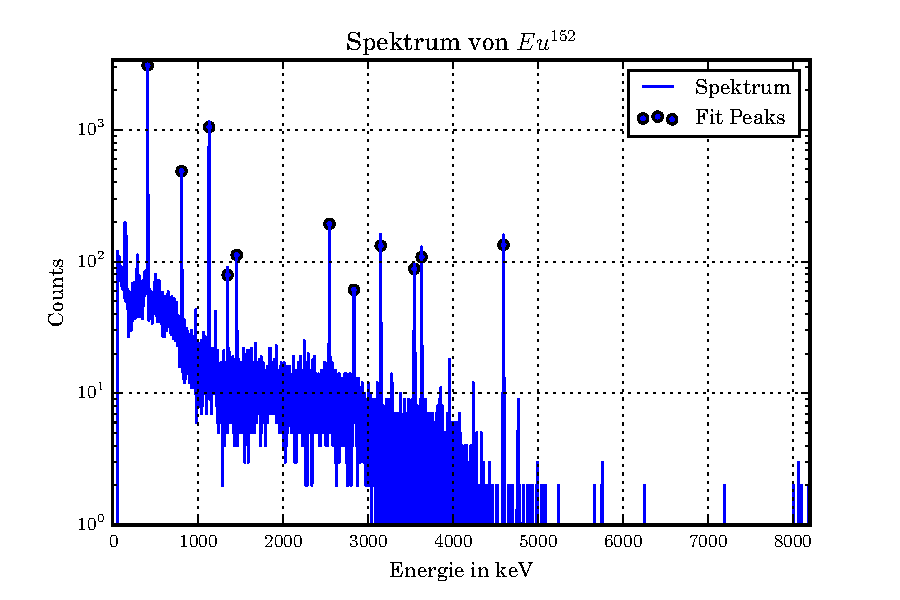
\includegraphics[width=\textwidth]{./build/SpektEu.pdf}
   \caption{Spektrum des Eu$^{152}$ zur Bestimmung der Effizienz des Detektors}
  \label{fig:SpekCs}
\end{figure}
Die Aktivität $A_\text{Eich}$ der verwendeten $^{152}$Europium betrug am 01.10.2000
\begin{equation}
  A_\text{Eich} = (\num{4130 +- 60}) \, \text{Bq}
  \label{eqn:AktEu}
\end{equation}
und die Halbwertszeit
\begin{equation}
  \tau_{1/2} = (\num{4943 +- 5}) \, \text{Tage} \ . \text{\cite{V18}}
  \label{eqn:halb}
\end{equation}
Anhand des exponentiellen Zerfallsgesetztes
\begin{equation}
  A(t) = A_\text{Eich} \cdot \exp \left(\frac{\ln(2)}{\tau_{1/2}} \, t \right)
  \label{eqn:zerfG}
\end{equation}
lässt sich mittels der Zeitdifferenz
\begin{equation}
  \Delta t = 5938 \text{Tage}
\end{equation}
zwischen der geeichten Aktivität und dem Tag der Durchführung der Messung (09.01.2017) eine Aktivität von
\begin{equation}
  A_\text{Durch} = (\num{1796 +- 26}) \, \text{Bq}
  \label{eqn:AktEEu}
\end{equation}
berechnen. Es wird versucht den Abstand zwischen Quelle und Detektor mittels eines Stabes, welcher bei der Justage der Quelle als Abstandsmaß dazwischen gespannt wird, konstant zu halten. Der Abstand beträgt
\begin{equation}
  a = (\num{8,8 +-0,3}) \, \text{cm}
\end{equation}
und der Radius $r$ des Detektors
\begin{equation}
  r = 2,25 \, \text{cm}
\end{equation}
wird der Anleitung \cite{V18} entnommen. Aus diesen lässt sich durch einsetzen in Formel \ref{eqn:Raumwinkel} ein Raumwinkel $\Omega$ von
\begin{equation}
  \Omega = \num{0,196 +- 0,021}
  \label{eqn:Raum}
\end{equation}
berechnen. Der Raumwinkel $\Omega$ ist jedoch nur unter vorbehalt zu verwenden, da der Abstand zwischen Quelle und Detektor kleiner als 10 cm ist und dies nicht mehr im Gültigkeitsbereich der Formel \ref{eqn:Raumwinkel} liegt. Aus dem Raumwinkel $\Omega$, der Wechselwirkungswahrscheinlickeit $W$, der Aktivität $A_\text{Durch}$ sowie der effektiven Messzeit lässt sich nach Formel \ref{eqn:Zählergebnis} die Effizienz $Q$ berechnen. Die Ergebnisse in Abhängikeit der Energie sind in Tabelle \ref{tab:CsSpekt} aufgeführt.
\begin{table}
  \centering
  \begin{tabular}{c| c c c}
     \toprule
    	Energie $E_{\gamma}$ / keV& Emissionwahrscheinlichkeit / \% \cite{V18}& Counts & Effizienz / \% \\
     \midrule
     121,78  &28,6 &\num{12180 +- 280} 	& ---	\\
     244,70  &7,6  &\num{2180 +- 110} 	& \num{32,4 +- 3,8}	\\
     344,30  &26,5 &\num{5060 +- 74} 	& \num{21,5 +- 2,3} 	\\
     411,12  &2,2  &\num{440 +- 60} 	& \num{22,5 +- 3,8} 	\\
     443,96  &3,1  &\num{520 +- 60} 	& \num{18,7 +- 2,9} 	\\
     778,90  &12,9 &\num{1120 +- 50}	& \num{9,8 +- 1,1}	\\
     867,37  &4,2  &\num{420 +- 40} 	& \num{11,2 +- 1,5}	\\
     964,08  &14,6 &\num{960 +- 40} 	& \num{7,4 +- 0,9}	\\
     1085,90 &10,2 &\num{580 +- 40} 	& \num{6,4 +- 0,8}	\\
     1112,10 &13,6 &\num{770 +- 30} 	& \num{6,4 +- 0,7}	\\
     1408,00 &21,0 &\num{900 +- 35} 	& \num{4,8 +- 0,6}	\\
     \bottomrule
  \end{tabular}
  \caption{Messwerte zur Berechnung der Effizienzfunktion des Detektors}
  \label{tab:Effi}
\end{table}

Um die Effizienz in dem folgenden Auswertungsteil \ref{sec:Q} zu berücksichtigen, wird diese in erster Näherung durch eine Potenzfunktion dargestellt. Bei dem Fit werden die Messwerte mit den Unsicherheiten der Effizienzen gewichtet.

\begin{figure}[H]
  \centering
  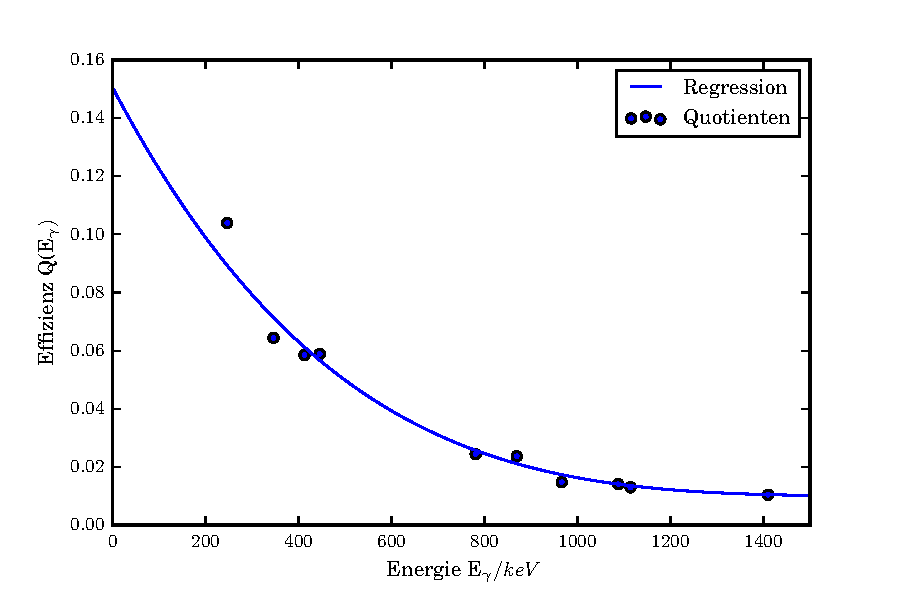
\includegraphics[width=\textwidth]{./build/Effizienz.pdf}
  \caption{Effizienz des verwendeten Germaniumdetektors}
  \label{fig:Efi}
\end{figure}

Die ermittelte Potenzfunktion zur Berechnung der Effizienz in Abhängigkeit der Energie, hat die Form
\begin{equation}
  Q(E_\gamma)=  a \cdot \left( E_\gamma \right)^{b} .
  \label{eqn:QCs}
\end{equation}
und der Fit ergibt die Parameter
\begin{eqnarray}
  a = (\num{1,2 +- 0,4}) \cdot 10^{-2} \\
  b = (\num{-1,07 +- 0,05}) \ .
\end{eqnarray}

\subsection{$^{137}$Cs-Strahler}
Für eine Messzeit von 2740 Sekunden werden Events für das Spektrum gesammelt. Aus diesem wird zunächst die Lage des Photopeaks bestimmt und das Compton-Kontinuum genauer untersucht. Anschließend wird geprüft ob der Photopeak einer Gaußverteilung entspricht. Zuletzt wird die Absorptionswahrscheinlichkeit des Detektors berechnet und Erklärungen für die Gestalt des Compton-Kontinums, sowie des Photopeaks gesucht.


\subsubsection{Photopeak}
In dem aufgenommenen Spektrum wird mittels der Funktion find\_peaks\_cwt aus der numpy Bibliothek die Lage des Photopeaks bestimmt. Das Ergebnis ist in Abbildung \ref{fig:SpekCS} zu sehen.
\begin{figure}
  \centering
  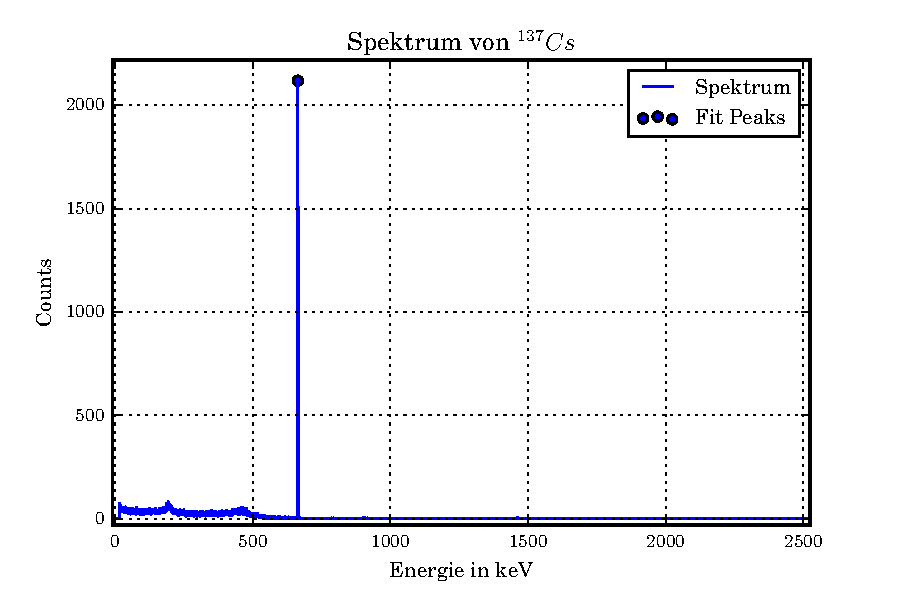
\includegraphics[width=\textwidth]{./build/SpektCS.pdf}
  \caption{Spektrum des Cs-Strahlers}
  \label{fig:SpekCS}
\end{figure}

Dabei wurde die X-Achse schon mittels der in Auswertungsteil \ref{sec:Kalb} Energie skaliert. Der Photopeak wird bei Energie von
\begin{equation}
  E_\gamma = (\num{661,5 +- 0,6}) \, \text{keV}
  \label{eqn:CsPhoto}
\end{equation}
detektiert. Im späteren Teil der Auswertung wird geprüft ob dem Photopeak eine gaußförmige Verteilung zu Grunde liegt.


\subsubsection{Compton-Kontinuum}
Für die weiteren Rechnungen wird zunächst die natürliche Energie $\varepsilon$ nach Formel \ref{eqn:normEnergie} eingeführt, welche
\begin{equation}
\varepsilon = \num{1,298 +- 0,001}
  \label{eqn:nE}
\end{equation}
beträgt. Aus der natürlichen Energie $\varepsilon$ des Strahlers kann die theoretische Lage der Comptonkante $E_\text{ComKan, theo}$ nach Formel \ref{eqn:Comptonkante} berechnet werden. Sie beträgt
\begin{equation}
  E_\text{ComKan, theo} = (\num{478,0 +- 0,6}) \, \text{keV}
  \label{eqn:KanTheo}
\end{equation}
Das Spektrum im Bereich des Compton-Kontinums ist in Abbildung \ref{fig:Compt} zu sehen.

\begin{figure}[htpb]
  \centering
  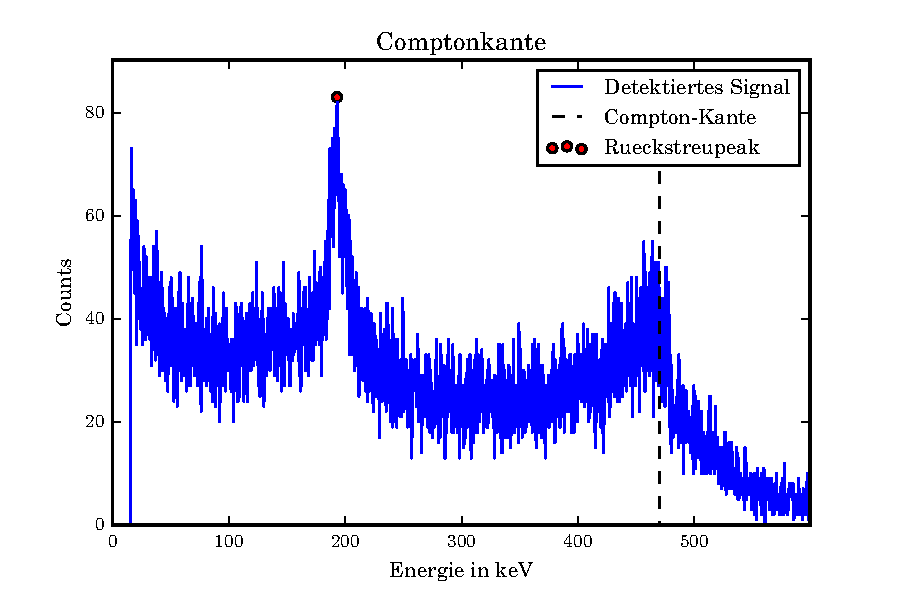
\includegraphics[width=\textwidth]{./build/Compton.pdf}
  \caption{Compton-Kontinuum mit Rückstreupeak und maximalen Energieübertrag}
  \label{fig:Compt}
\end{figure}

Aus dem Spektrum des Compton-Kontinuums wird der Rückstreupeak per Hand abgeschätzt. Dabei wird die Energie gesucht, bei der die Anzahl an Counts maximal wird. Aufgrund der statistischen Fluktuationen der Verteilung und dem Verlauf des Spektrums, kann nicht ganz eindeutig Identifiziert werden, ob die am häufigsten auftretende Energie auch dem Rückstreupeak entspricht. Dementsprechend wird der Fehler im Bereich der möglichen Energien des Rückstreupeaks bemessen. Die abgeschätzte Rückstreu-Energie beträgt
\begin{equation}
  E_\text{rück} = (\num{193 +- 10}) \, \text{keV} \ .
  \label{eqn:KanExp}
\end{equation}
Die Energie der maximalen Energieübertragung wird ebenfalls per Hand abgeschätzt, indem die Flanke gesucht wird bei der das Comptonkontinum einbricht und gegen Null strebt.
\begin{equation}
  E_\text{l,max} = (\num{470 +- 25}) \, \text{keV}
  \label{eqn:RückExp}
\end{equation}
Da auch die Compton-Kante nicht eindeutig identifizierbar ist, wird der Bereich der möglichen Energien als Fehler geschätzt.


\subsubsection{Verteilung des Photopeaks}
Um zu überprüfen ob der Photopeak gaußverteilt ist wird der Zusammenhang zwischen der Zehntelwertsbreite und der Halbwertsbreite überprüft. Dazu wird zunächst das Maximum $M$ bestimmt. Anschließend wird eine Linie in die Messwerte gelegt die dem $M/n$ fachen entspricht. Zwischen den jeweiligen Werten die am nächsten an der Linien des $M/n$ fachen liegt wird eine lineare Regression durchgeführt und der Punkt bestimmt bei dem die Regression den Wert $M/n$ angenommen hat. Die Punkte werden jeweils für die Seite links und rechts vom Maximum bestimmt und der Abstand dortzwischen ermittelt. Der Abstand wird als $1/n$-Wertsbreite bezeichnet.
Die Halbwertsbreite sowie die Zehntelwertsbreite sind in Abbildung \ref{fig:Halb} und \ref{fig:Zehntel} zu sehen.

\begin{figure}[h]
  \centering
  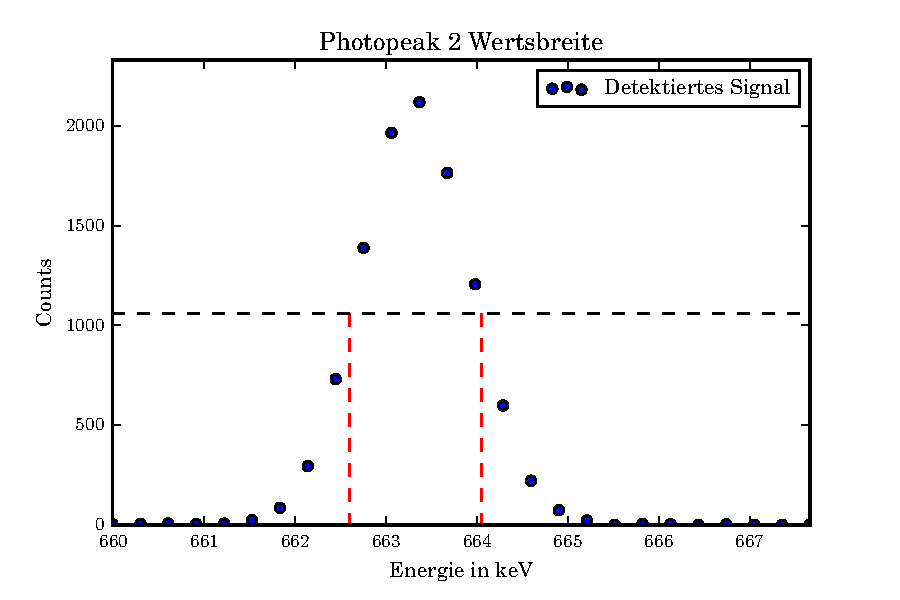
\includegraphics[width=\textwidth]{./build/2Wertsbreite.pdf}
  \caption{Halbwertsbreite}
  \label{fig:Halb}
\end{figure}

\begin{figure}[h]
  \centering
  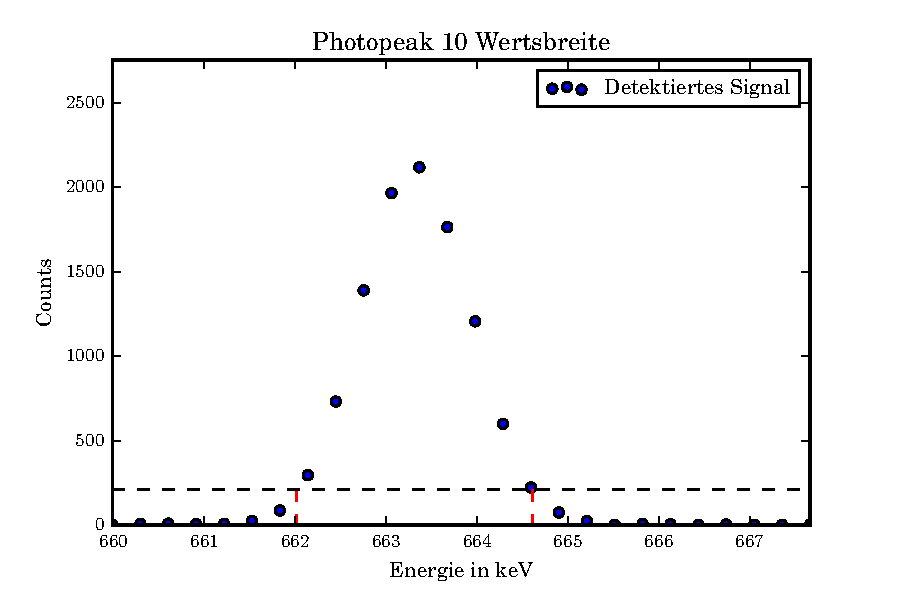
\includegraphics[width=\textwidth]{./build/10Wertsbreite.pdf}
  \caption{Zehntelwertsbreite}
  \label{fig:Zehntel}
\end{figure}
Aufgrund der Aproximation der 1/n-Wertsbreiten durch eine Grade der benachtbarten Spektrumpunkte wird der Fehler nach oben hin durch die Skalierung von Kanal und Energie, sowie der Annahme das die Messwerte der Poissonverteilung unterliegen, abgeschätzt. Die ermittelte Halbwertsbreite $\Delta E_{1/2}$ beträgt
\begin{equation}
  \Delta E_{1/2} = (\num{1,46 +- 0,63}) \, \text{keV}
\end{equation}
und die mittels Formel \ref{eqn:Halbwertsbreite} theoretische Halbwertsbreite
\begin{equation}
  \Delta E_{1/2 \text{, theo}} \approx 1,00 \, \text{keV}
  \label{eqn:HalbTheo}
\end{equation}
Mögliche Ursachen für die Abweichung der experimentellen Halbwertsbreite von der theoretischen werden in der Diskussion aufgeführt. Die Zehntelwertsbreite $\Delta E_{1/10}$ beträgt
\begin{equation}
  \Delta E_{1/10} = (\num{2,60 +- 0,39}) \, \text{keV}
\end{equation}
Im Falle einer Gaußverteilung müsste das Verhältniss zwischen Halb- und Zehntelwertsbreite
\begin{equation}
  \frac{\Delta E_{1/10}}{\Delta E_{1/2}} = 1,823
\end{equation}
seien. Das Verhältniss zwischen den experimentell bestimmten Breiten ist
\begin{equation}
  \frac{\Delta E_{1/10}}{\Delta E_{1/2}} = \num{1,8 +- 0,8}
  \label{eqn:Ver}
\end{equation}
Daraus wird geschlossen das hinreichend viele Werte genommen worden sind, sodass die Poissonverteilung in die Gaußverteilung übergeht.

\subsubsection{Absorptionswahrscheinlichkeit im Detektor}
Aus Abbildung \ref{fig:Extink} kann der Extinktionskoeffizient $\mu$ für Germanium entsprechend der auftretenden Effekte abgelesen werden. Der Extinktionskoeffizient für den Photoeffekt bei einer Energie von ca. 650\,keV ist in etwa
\begin{equation}
  \mu_\text{Photo} = 0,007 \, \text{cm} ^{-1} \ .
  \label{eqn:muPhoto}
\end{equation}
Unter Verwendung von Formel \ref{eqn:absorption} lässt sich die Absorptionswahrscheinlichkeit durch den Photoeffekt auf
\begin{equation}
  p_\text{Absorp, Photo} \approx 3,1 \, \%
  \label{eqn:AbsorpPhoto}
\end{equation}
berechnen. Die Anzahl der Ereignisse $I_\text{Photo}$ im Photopeak wird durch das Integrieren eines Gaußfits berechnet, bei dem als Unsicherheit die Standardabweichung des Fittes genommen wird.
\begin{equation}
  I_\text{Photo} = \num{10550 +- 80}
  \label{eqn:iPhoto}
\end{equation}
Der Extinktionskoeffizient beim Comptoneffekt bei ca. 650\,keV beträgt
\begin{equation}
  \mu_\text{Compt} = 0,4 \, \text{cm} ^{-1} \ .
  \label{eqn:muCompt}
\end{equation}
Daraus errrechnet sich eine Absorptionswahrscheinlichkeit von
\begin{equation}
  p_\text{Absorp, Compton} \approx 70 \, \% \ .
  \label{eqn:AbsorpComp}
\end{equation}
Der Inhalt des Comptoneffekts beträgt
\begin{equation}
  I_\text{Compton} = \num{50000 +- 2500} 
  \label{eqn:iComp}
\end{equation}
und wird durch die Summation der einzelnen Ereignisse bis zu der theoretischen Compton-Kante genommen. Unter der Annahme, dass der Wirkungsquerschnitt der Paarbildung für Energien unterhalb von 700\,keV vernachlässigt wird, beträgt die normierte theoretische Wahrscheinlichkeit
\begin{equation}
  p_\text{Absorp, Photo} \approx 4,2 \% \text{ und } p_\text{Absorp, Compton} \approx 95,8 \% \ .
  \label{eqn:pNorm}
\end{equation}
Die normierten Events setzen sich zu
\begin{equation}
  Z_\text{Photo} \approx 17,4 \% \text{ und } Z_\text{Compton} \approx 82,6 \%
  \label{eqn:expNorm}
\end{equation}
zusammen. Die Annahme, dass jedes Photon nur einmal in dem Detektor wechselwirkt ist allgemein nicht richtig. Ein Photon kann nach einem Compton-Stoß weitere Wechselwirkungen durchführen. Ergibt die Summe aller Wechselwirkungen eines Photons die Energie $E_\gamma$, so wird das Photon fälschlicher weise dem Photopeak zugeordnet. Dadurch wird ein höherer Photopeak gemessen, als berechnet wird.
\subsection{Aktivitätsbestimmung der verwendeten $^{133}$Ba-Quelle}
Zur Bestimmung der Aktivität der verwendeten $^{133}$Bariumquelle wurde das in Abbildung \ref{fig:BA} zu sehende Spektrum bei einer Messzeit von 3595 Sekunden aufgenommen.
\begin{figure}[H]
  \centering
  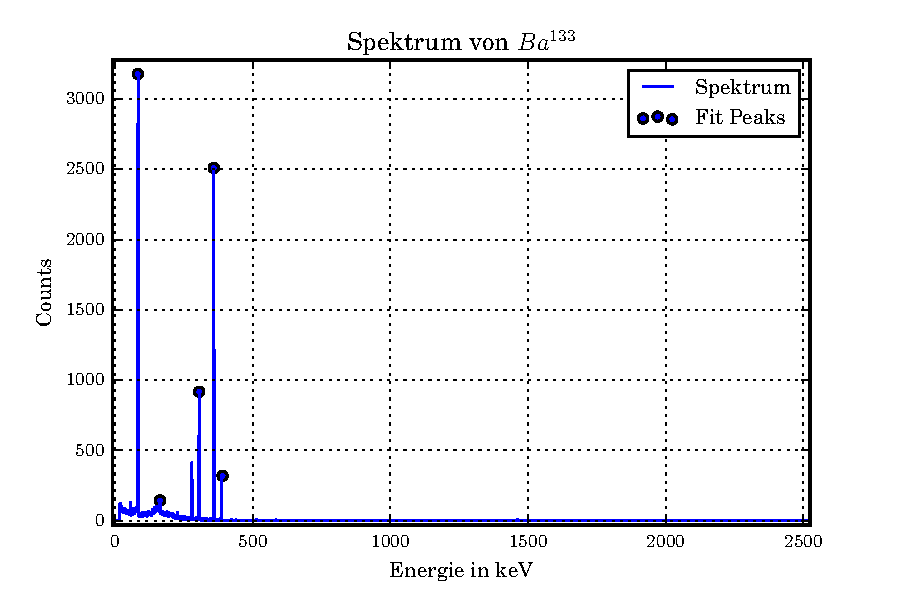
\includegraphics[width=\textwidth]{./build/SpektBa.pdf}
  \caption{Spektrum der verwendeten $^{133}$Bariumquelle zur Bestimmung der Aktivität}
  \label{fig:BA}
\end{figure}
Das Zählergebnis der Spektrallinien $Z$, die Effizienzen $Q(E_\gamma)$ und die Wechselwirkungswahrscheinlickeit $W$ sind in Tabelle \ref{tab:Ba} zusammen mit den kalibrierten Energien aufgetragen. Der Raumwinkel wurde bereits in Kapitel \ref{sec:Q} bestimmt und beträgt \\
$\Omega = \num{0,196 +- 0,021}$ .
\begin{table}
  \centering
  \caption{Aktivität in Abhängigkeit der Energie sowie der Effizienz und der Wechselwirkungswahrscheinlichkeit}
  \begin{tabular}{c c c c c}
    \toprule
	$E_\gamma$ / keV & $Z$ & $Q(E_\gamma)$ & $W$ / \%  & $A / (1/s)$\\
    \hline
    \num{160,6 +- 2,5}	& \num{2200 +- 400}	&\num{0,514 +- 0,009}      	& 0,6	&\num{12700 +- 2600}      \\
    \num{276,3 +- 0,5}  & \num{1760 +- 60}	&\num{0,2893 +- 0,0006} 	& 7,16 	&\num{1520 +- 170}  	\\
    \num{302,9 +- 0,5}	& \num{3350 +- 60} 	&\num{0,2620 +- 0,0004} 	& 18,3	&\num{1320 +- 140}   	\\
    \num{356,0 +- 0,5}	& \num{10120 +-	80}	&\num{0,2204 +- 0,0003} 	& 62,1	&\num{1320 +- 140}  	\\
    \num{383,8 +- 0,5}	& \num{1390 +- 30}	&\num{0,2032 +- 0,003} 		& 8,9	&\num{1370 +- 150}  	\\
    \bottomrule
  \end{tabular}
  \label{tab:Ba}
\end{table}
Durch umstellen der Gleichung \ref{eqn:Zählergebnis} nach A lässt sich die Aktivität der Probe ermitteln wobei die Zählergebnisse noch einmal durch die Messdauer geteilt werden müssen. Die Aktivitäten der einzelnen Energien sind in Tabelle \ref{tab:Ba} aufgetragen. Bei einer Energie $E_\gamma = (\num{160,6 +- 2,5})$ keV ist die Detektionswahrscheinlickeit des Peaks so gering, dass in dem  Zählergebnis zum größten Teil die Zählergebnisse des Compton-Kontinuums gemessen werden, anstelle der Spektrallinie. Aufgrund dessen wird dieser Wert bei der Bestimmung der mitteleren Aktivität vernachlässigt. Das gemittelte Ergebniss beträgt
\begin{equation}
  A = (\num{1380 +- 50}) \, \text{Bq}
  \label{eqn:aktBq}
\end{equation}
\subsection{Zerfallsreihe des unbekannten Minerals}
Es wird versucht aus dem in einer Messzeit von 2716 Sekunden aufgenommen Linienspektrum des verwendeten Minerals auf die Zerfallsreihe der Probe zu schließen. Das Linienspektrum des Minerals ist in Abbildung \ref{fig:Stone} zu sehen.
\begin{figure}[h]
  \centering
  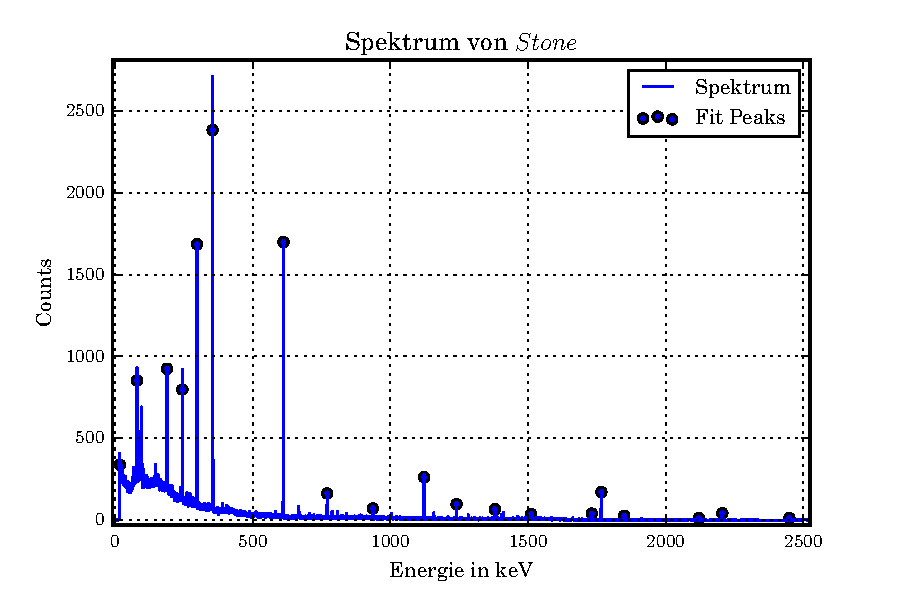
\includegraphics[width=\textwidth]{./build/SpektSt.pdf}
  \caption{Spektrum von verwendeten Mineral}
  \label{fig:Stone}
\end{figure}
Mit Hilfe der find\_peaks\_cwt der scipy Biblothek werden in dem Spektrum die Peaks gesucht. Die Energien $E_\text{Peak}$ bei denen die Peaks vorgefunden werden sind in Tabelle \ref{tab:Stone} aufgeführt. Diese werden mit den Energien der $^{232}$Thorium- und $^{238}$Uran-Zerfallsreihe $E_\text{Zerfallsreihe}$ verglichen.
\begin{table}
  \centering
  \caption{Vergleich des Spektrums mit natürlichen Zerfallsreihen}
  \begin{tabular}{c c c c}
    \toprule
    $E_\text{Peak}$ / keV & $E_\text{Zerfallsreihe} /keV$ & Em-Wahrscheinlichkeit / \% & Zerfallsreihe \\
    \midrule
    \num{77,3+-3,0}	& ---	& ---	& ---	\\
    \num{186,0+-0,9}	& 186	& 4	&Uran($^{226}$Ra)	\\
    \num{242,1+-0,6}	& 242	& 4	&Uran($^{214}$Pb)	\\
    \num{295,2+-0,5}	& 295	& 19	&Uran($^{214}$Pb)	\\
    \num{352,0+-0,5}	& 352	& 36	&Uran($^{214}$Pb)	\\
    \num{609,3+-0,6}	& 609	& 47	&Uran($^{214}$Bi)	\\
    \num{768,3+-0,8}	& 769	& 5	&Uran($^{214}$Bi)	\\
    \num{934,1+-1,0}	& 935	& 3	&Uran($^{214}$Bi)	\\
    \num{1120,4+-0,7}	& 1120	& 17	&Uran($^{214}$Bi)	\\
    \num{1238,3+-0,8}	& ---	& ---	& ---	\\
    \num{1377,7+-0,8}	& 1378	& 5	&Uran($^{214}$Bi)	\\
    \num{1509,3+-1,2}	& 1509	& 2	&Uran($^{214}$Bi)	\\
    \num{1729,8+-0,9}	& 1728	& 3	&Uran($^{214}$Bi)	\\
    \num{1764,4+-0,9}	& 1764	& 17	&Uran($^{214}$Bi)	\\
    \num{1847,3+-1,0}	& ---	& ---	& ---	\\
    \num{2118,7+-1,2}	& ---	& ---	& ---	\\
    \num{2204,0+-0,9}	& 2204	& 5  	&Uran($^{214}$Bi)	\\
    \num{2447,5+-0,7}	& ---	& ---	& ---	\\
    \bottomrule
  \end{tabular}
  \label{tab:Stone}
\end{table}
Auffällig ist das erst Zerfälle oberhalb einer Emmisionswahrscheinlichkeit von $>2\%$ detektiert werden können, da diese sonst bei der Menge an Events nur schwer vom Rauschen/dem Compton-Kontinuum auseinander zu halten sind. Dabei treten die Isotope $^{226}$Ra, $^{214}$Pb und $^{214}$Bi in dem Spektrum auf. Der mögliche Zerfall von $^{214}$Bi in $^{210}$Pb kann nicht detektiert werden, da die Aluminiumhülle des Germaniumdetektors diesen in dem Bereich bis 50 keV abschirmt. Desweiteren können keine weiteren Zerfallsprodukte der Uran-Zerfallsreihe mehr detektiert werden. Zerfallsprdoukte treten nach Abgleich der natürlichen $^{232}$Thorium-Zerfallsreihe \cite{V18} nicht auf.
Desweiteren treten in dem Spektrum noch Zerfälle auf, die keinem Isotop eindeutig zugeordnet werden können. Diese stammen vermutlich aus einer anderen Zerfallsreihe.
